\section{Evaluation}
 \label{sec:evaluation}
 
 We implemented a prototype of \name in Python. 
 For a given workload, \name outputs Quagga configurations~\cite{quagga}. 
 We use the the solver Gurobi~\cite{gurobi} 
 to solve the linear constraints generated by \name.
  In this section, we evaluate \Name using
%\loris{really don't like the word realistic}
enterprise-scale data
center fat-tree topologies~\cite{fattree} of different 
sizes. 
Specifically, we ask the folloqing questions.\footnote{All experiments were conducted using a
32-core Intel-Xeon 2.40GHz CPU machine and
128GB of RAM.}

\vspace{2mm}
\begin{tabular}{p{0.5cm}p{0.88\textwidth}}
\textbf{Q1} &  What is the performance of \name on different synthesis workloads? (\secref{sec:ospfeval})\\

\textbf{Q2} & How resilient are the configurations  generated by \name? (\secref{sec:reseval})\\

\textbf{Q3} &  Can \name get higher resilience when it is allowed to try different domain assignments? (\secref{sec:mcmceval})
\end{tabular}


\subsection{Single Domain End-to-end Performance with Genesis}\label{sec:ospfeval}


We evaluate the end-to-end performance of our tool
on a  fat-tree 
topology comprising of 45 routers
and a single OSPF domain. 
The size of the topology is consistent with operator preferences to restrict
the size of a domain to under 50 routers (OSPF does not scale
well as domain size increases).
We use \todo{name} to refer to the algorithm that handles complex policies and
can synthesize policy-compliant
configurations with few static routes (\secref{sec:config-synthesis})
and 
\todo{name} to refer to the algorithm that handles waypoint policies and
can synthesize policy-compliant
configurations with high policy-resilience (\secref{sec:waypointres}).

We consider two classes of policies.
Our first class contains complex isolation policies that 
existing tools cannot handle; for this class we can only evaluate algorithm \todo{alg1}.
Our second class consists of
 waypoint policies of the form described in Section~\ref{sec:waypointres});
for this class we evaluate both \todo{alg1} and \todo{alg2}.
For each algorithm  we evaluate how much time is spent
calling \genesis to generate policy-compliant paths
and how much time \name takes to generate configurations from such paths.


%of the path-compliance synthesis algorithm for tenant 
%isolation workloads, and single-path waypoint-compliance 
%synthesis for varying number of waypoint policies.


\begin{wrapfigure}[14]{r}{0.6\columnwidth}
	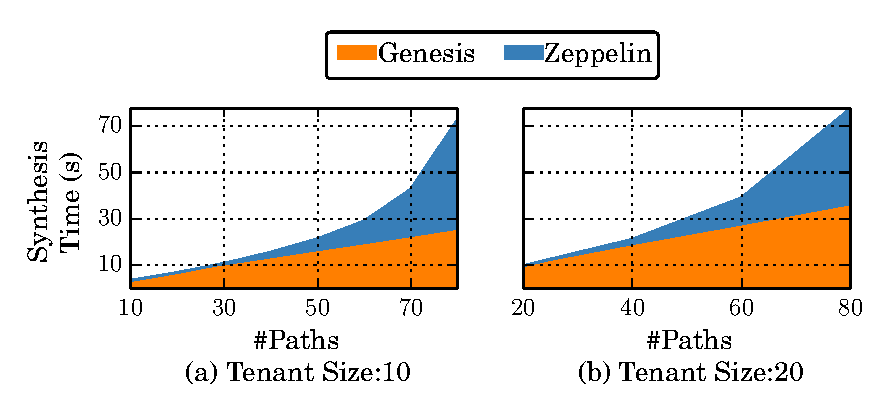
\includegraphics[width=0.58\columnwidth]{figures/ospfisolation.eps}
	%	\subfloat[Number of Route Filters]
	%	{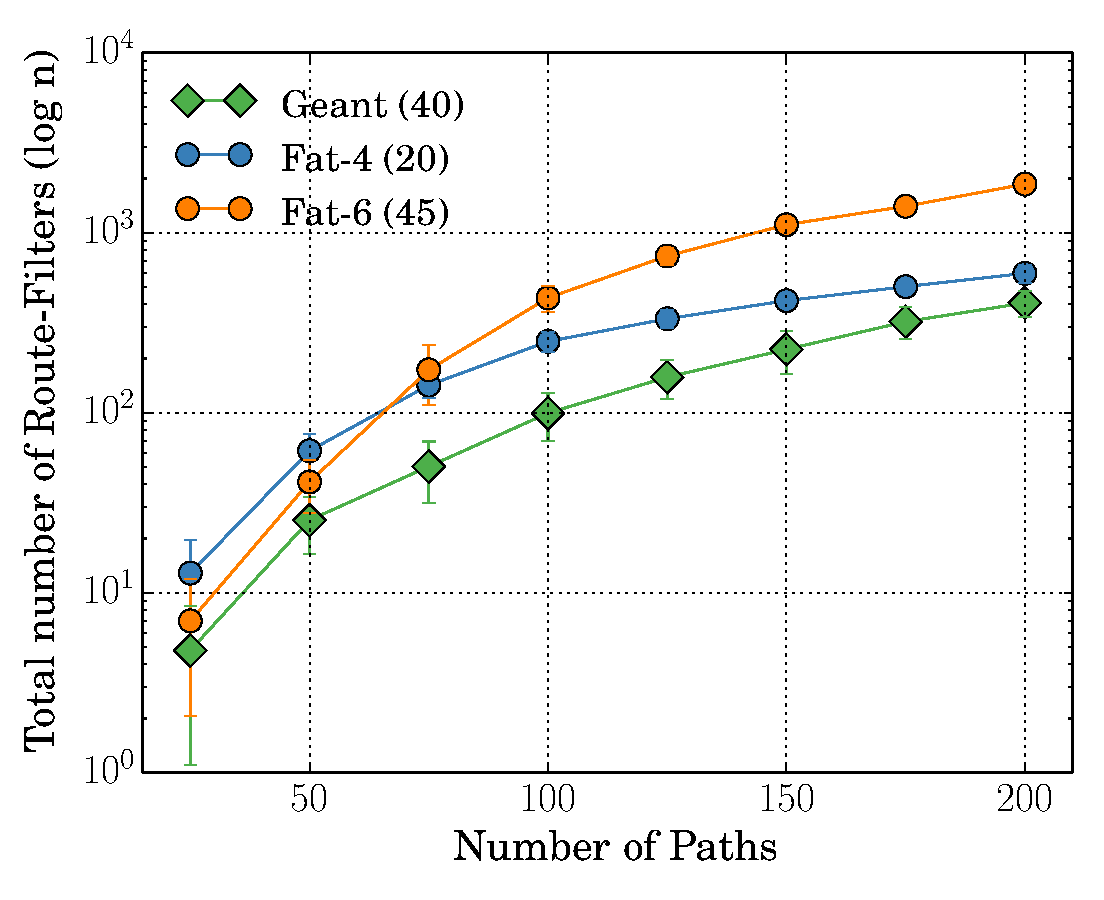
\includegraphics[width=0.33\columnwidth]{figures/ospfRF.eps}}
	%	\subfloat[Endpoint Resilience]
	%	{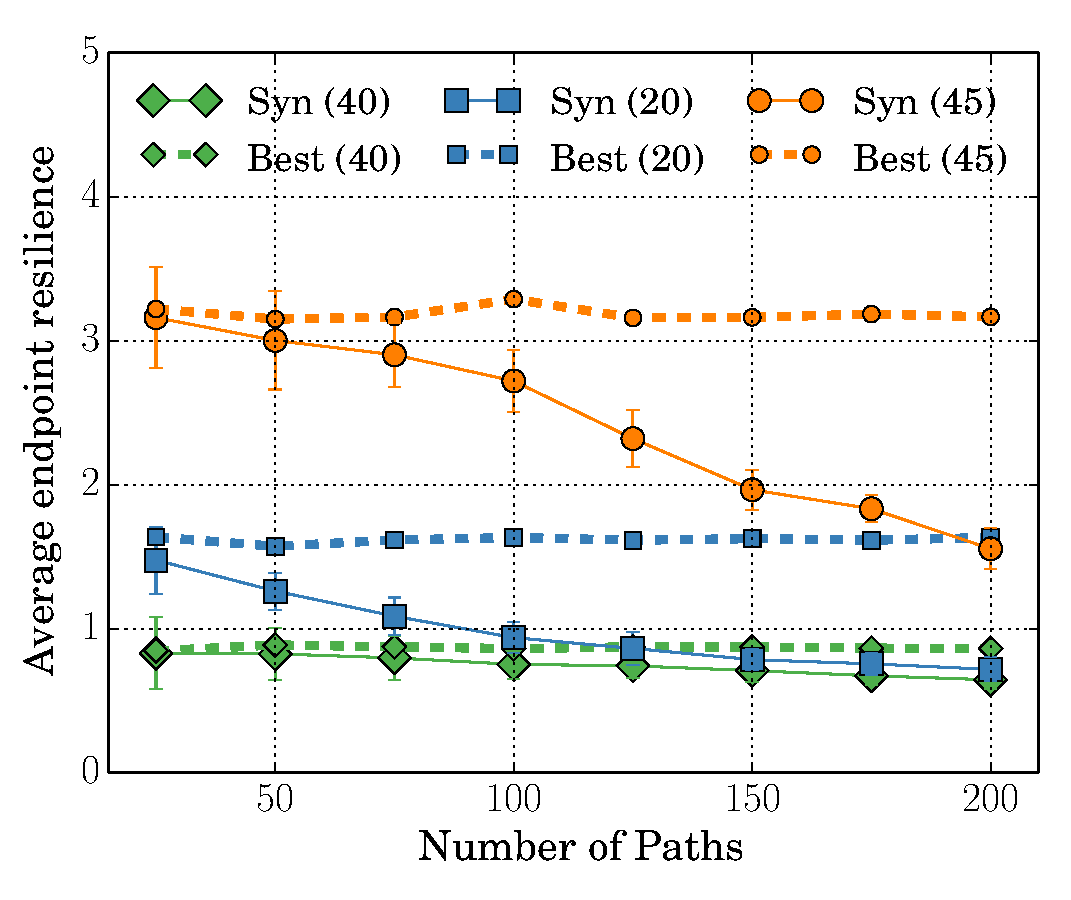
\includegraphics[width=0.32\columnwidth]{figures/ospfAvgRes.eps}}
	\vspace{-8pt}
	\compactcaption{\label{fig:ospfisolation}
		End-to-end synthesis time for isolation workloads over the range of destinations and different tenant sizes.}
\end{wrapfigure}
\paragraph{Isolation Policies.}
We generate policies that operate 
on a multi-tenant topology with 
 different tenants.
Within a  group of tenants, we add a policy to ensure
each path  (with randomly generated endpoints)
is isolated from other paths of the same tenant group.
Here, isolation  prevents interference by other traffic belonging to
same tenant.  
\todo{I removed 1-PC from text not sure if used in graphs or later}
 
For each 
workload, we have $n$ tenant groups (between \todo{X and Y}), 
each group comprised of $g$ destinations (between 10 and 20). 
\Cref{fig:ospfisolation} 
shows the synthesis time 
for \todo{alg1}.
The x-axis shows the number of \loris{what paths} paths $n * g$. 
 As the number of tenants increase, time to 
synthesize the data plane increases linearly as we only 
consider isolation policies within tenants, not amongst paths 
of different tenants. Meanwhile, time taken to synthesize 
OSPF configurations increases exponentially with increasing 
number of tenants due to the exponential complexity of computing 
the unsat-cores; with increasing number of 
paths, \todo{alg1} needs to add more static routes  and requires more iterations of the unsat-core learning
procedure. 
For this workload, our tool can
synthesize configurations for 4 tenants, each with
20 destinations in 77 seconds, where \genesis takes 35 seconds and
\name takes 42 seconds on average. 

\todo{tool is zeppelin as well as genesis, we should change terminology}

\begin{wrapfigure}{r}{0.6\columnwidth}
	\begin{center}
		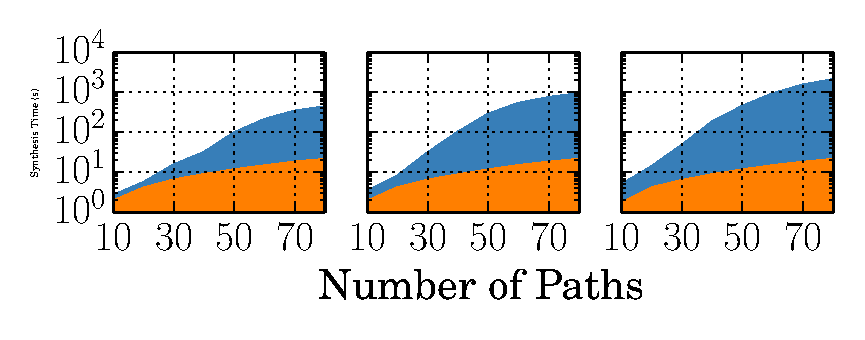
\includegraphics[width=0.6\columnwidth]{figures/ospfwaypoint.eps}
		%	\subfloat[Number of Route Filters]
		%	{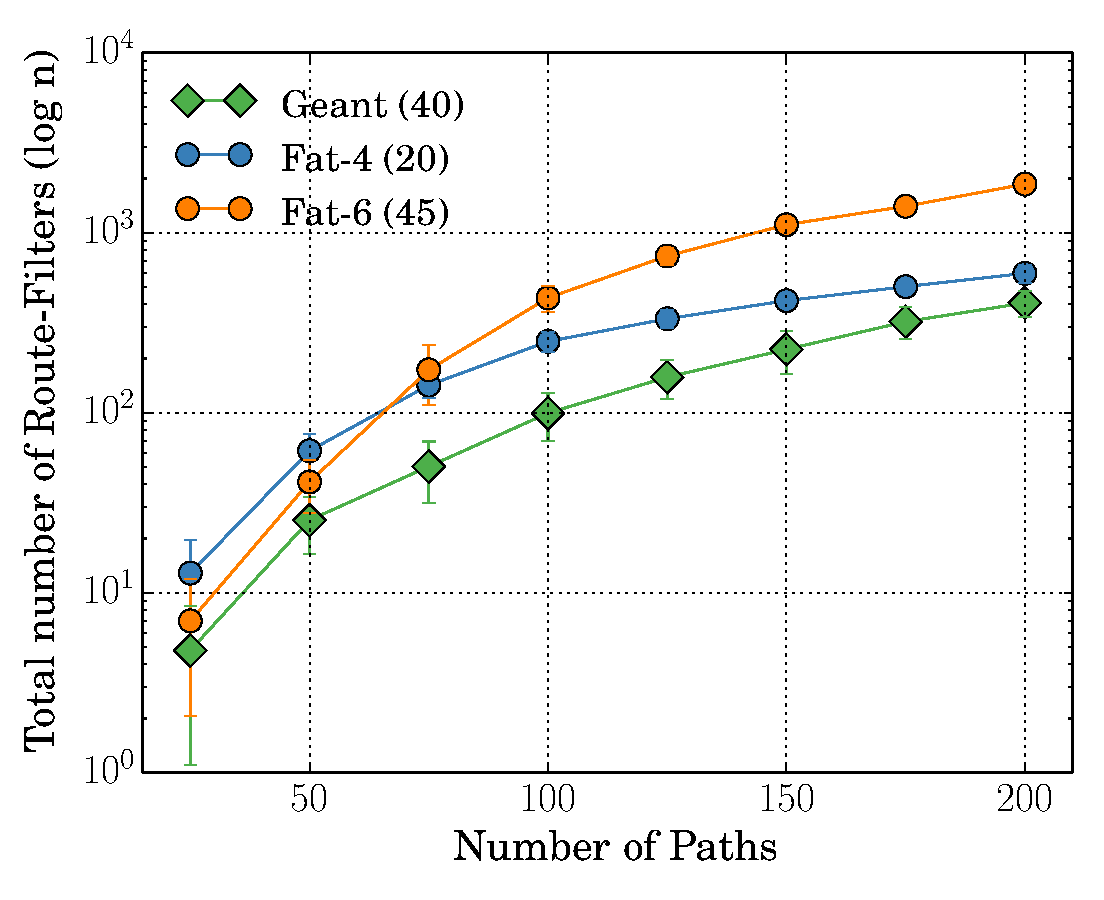
\includegraphics[width=0.33\columnwidth]{figures/ospfRF.eps}}
		%	\subfloat[Endpoint Resilience]
		%	{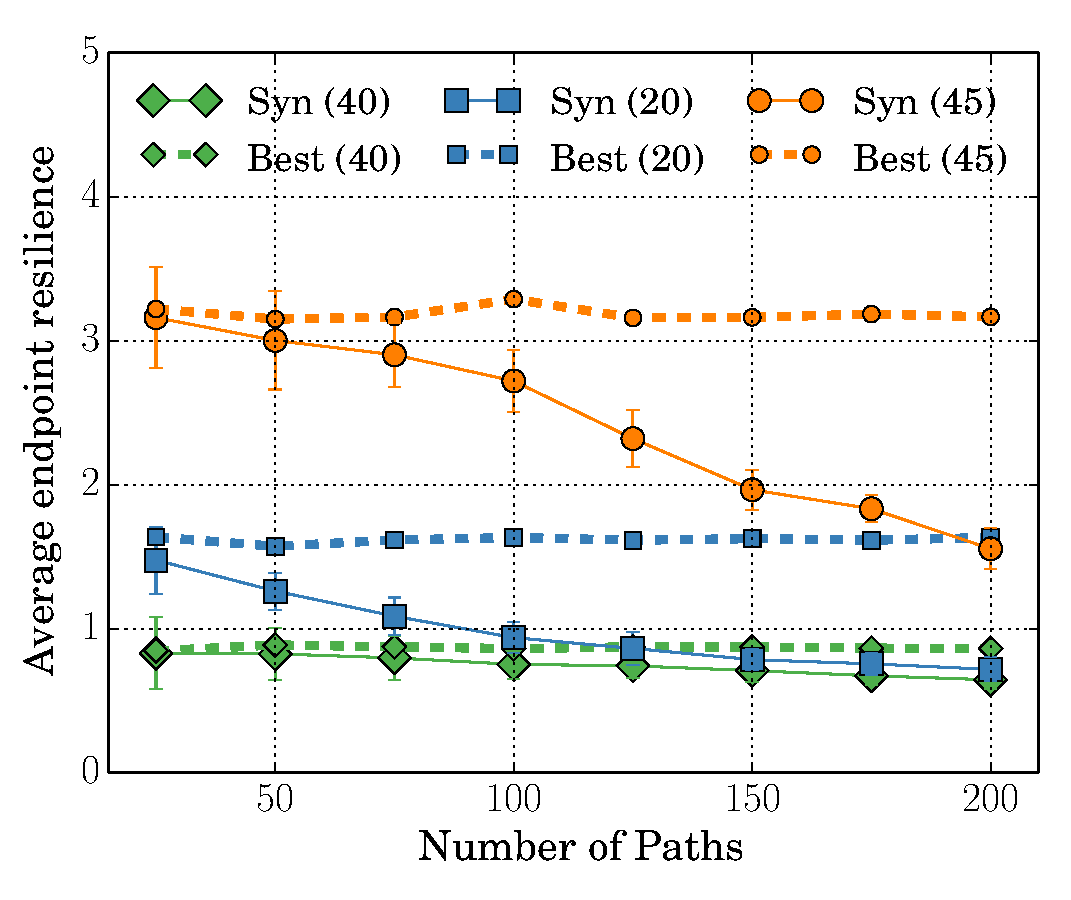
\includegraphics[width=0.32\columnwidth]{figures/ospfAvgRes.eps}}
		\compactcaption{\label{fig:ospfwaypoint}
		End-to-end synthesis time (log (s)) for waypoint policy workloads for varying 
		number of paths and different number of waypoint sets.}
	\end{center} 
\end{wrapfigure}
\paragraph{Waypoint Policies.}
We generate waypoint policy 
workloads with varying number of destination IP addresses and 
waypoint sets as follows. We create waypoint sets by generating
random sets of routers of size 3 and vary the number of 
unique waypoint sets in the topology across 2, 5, and 10 sets. 
\todo{previous sentence is weird?}
Each waypoint set can be 
viewed as a class of replicated middleboxes (for e.g., firewall).
We randomly generate policies that map each destination to one of the waypoint sets. 

%Genesis generates a single path for each 
%destination, and \name synthesizes waypoint-compliant OSPF 
%configurations ((referred to as 1-WC) ) 
%using the waypoint policies and paths generated by Genesis.  

\todo{rewrite following as alg 1 and alg2}
\Cref{fig:ospfwaypoint} shows the end-to-end synthesis
 time (log scale) for varying number of destinations paths and the 
 number of unique waypoint sets. Since, synthesizing paths
 for waypoint policies can be synthesized independently,
Genesis synthesis time is $<20s$. \name's 1-WC synthesis 
time increases as we increase the number of waypoint sets,
as we need to add constraints corresponding to $D_s^t(\waypt)$ 
for each set, and thus, computing the unsat-core in each
iteration to find a static route is more expensive with increasing
number of sets. For 5 waypoint sets, \name takes 300 
seconds on average to synthesize waypoint-compliant configurations. 


In summary, the answer to \textbf{Q1} is that, for realistic workloads,
\textbf{\name can synthesize configurations for medium size
topologies} less than five minutes.

%\begin{table}{l}{8em}
%	\begin{footnotesize}
%		\begin{center}
%			\begin{tabular}{P{10em}| P{4em} | P{4em} | P{4em} | P{4em}}
%				Synthesis Type & Number of Packet Classes & Avg. Synthesis time (s) & Avg. Number of Resilient Classes & Ratio of Static Routes \\
%				\hline
%				1-Resilient Waypoint & 10 & 122.16 & 7.13 & 7/100\\
%				Waypoint & 10 & 7.85 & 0.3 & 7/100\\
%				1-Resilient Waypoint & 20 & 122.16 & 7.1 & 7/100\\
%				Waypoint & 20 & 7.85 & 0.3 & 7/100\\
%				1-Resilient Waypoint & 40 & 122.16 & 7.1 & 7/100\\
%				Waypoint & 40 & 7.85 & 0.3 & 7/100\\
%			\end{tabular}
%		\end{center}
%		\compactcaption{Average synthesis time per class for waypoint policies with increasing number of waypoints. } \label{tab:waypointeval} 
%	\end{footnotesize}
%\end{table} 

\subsection{Resilience Performance of Intra-domain Synthesis} \label{sec:reseval}
\paragraph{Connectivity-resilience.}~~~
We now evaluate the resilience of configurations 
of \name's intra-domain synthesis (1-PC).
For this, 
we consider the path-compliance isolation workload for
varying number of paths 
in \secref{sec:ospfeval} and benchmark the connectivity-
resilience obtained over a baseline path-compliance 
configuration 
where we use static routes for all links in the path and 
assign OSPF edge weights randomly. For these workloads,
\name on average places 
$(8 \pm 0.5)$\% of the static routes as 
compared to the baseline configuration. 
\Cref{fig:ospfbaselineresilience}
shows the plot of connectivity-resilience scores for 
1-PC configurations over the baseline configurations. 
1-PC provides an average connectivity-resilience score 
of 0.95 over the baseline score 
of 0.85.

\begin{wrapfigure}{r}{0.20\columnwidth}
	\begin{center}
		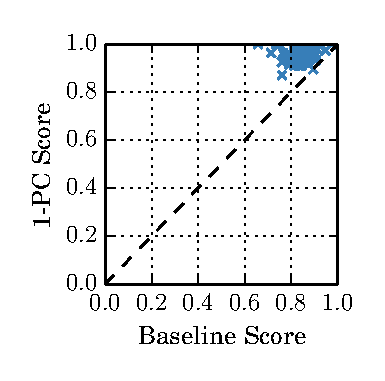
\includegraphics[width=0.20\columnwidth]{figures/ospfbaselineresilience.eps}
		%	\subfloat[Number of Route Filters]
		%	{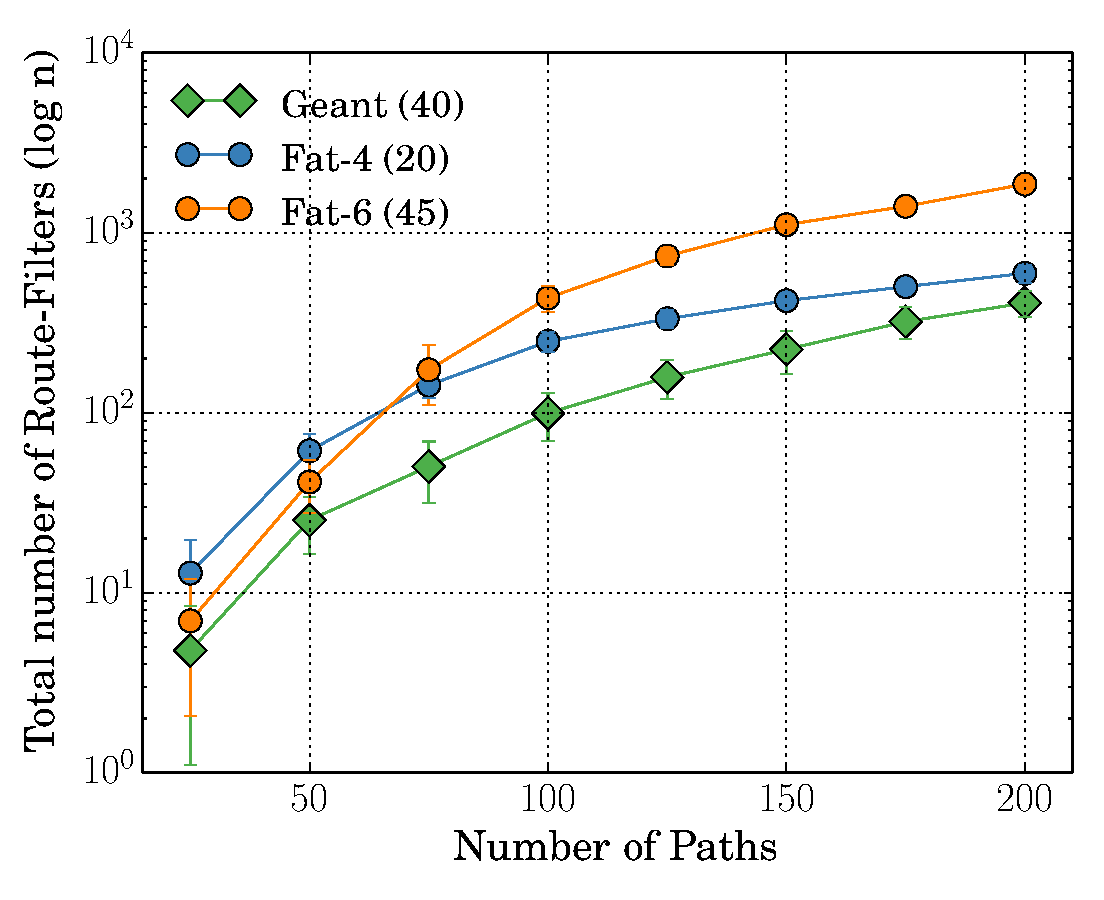
\includegraphics[width=0.33\columnwidth]{figures/ospfRF.eps}}
		%	\subfloat[Endpoint Resilience]
		%	{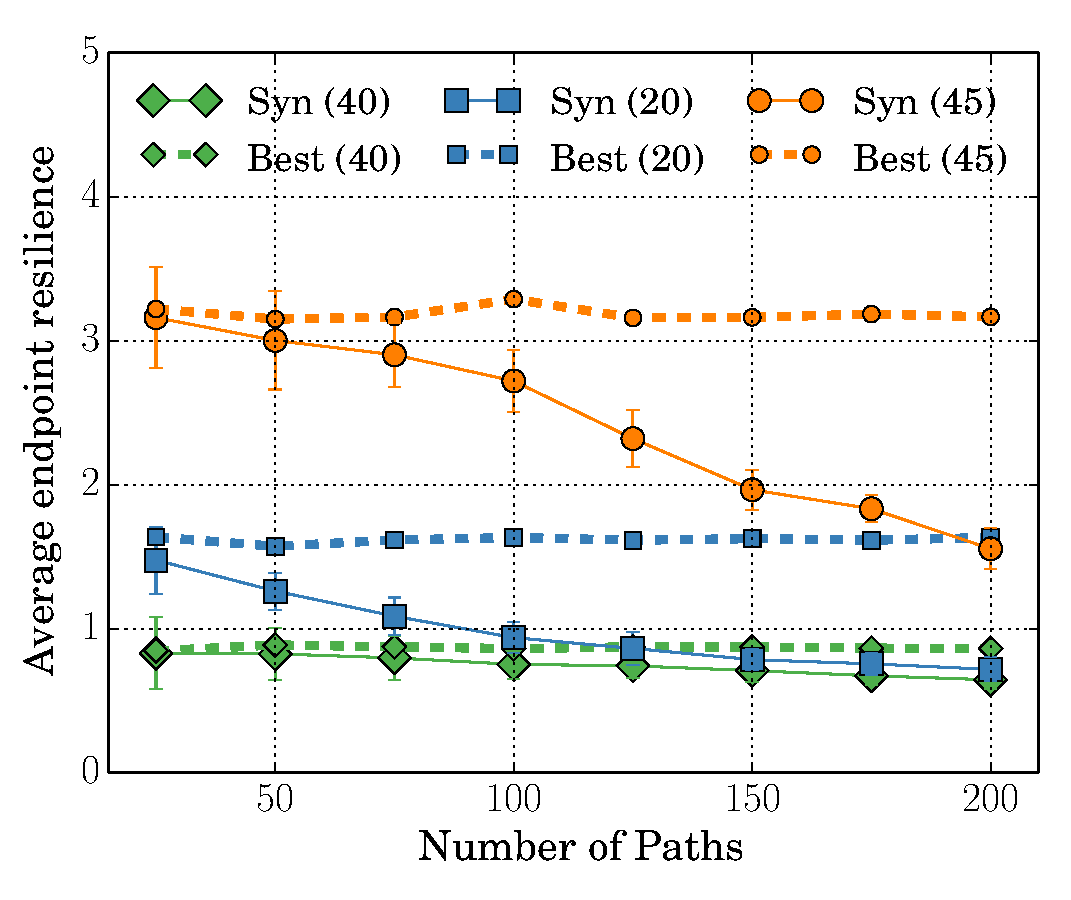
\includegraphics[width=0.32\columnwidth]{figures/ospfAvgRes.eps}}
		\compactcaption{\label{fig:ospfbaselineresilience}
			Connectivity-resilience for 1-PC configurations compared to the baseline 
			configurations.}
	\end{center} 
\end{wrapfigure}


\paragraph{Resilient Waypoint Compliance.}~~~
We now evaluate the resilience obtained by \name's
resilient waypoint-compliance synthesis (referred to as 2-WC)
described in \secref{sec:waypointres}
for the waypoint policy workload with 5 unique waypoint sets 
over two cases: (1) 1-PC: \name uses a single waypoint path
synthesized by Genesis for each policy 
and synthesizes a path-compliant configuration, and 
(2) 1-WC: \name sythesizes a waypoint-compliant configuration
using a single waypoint-path from Genesis. For these 
experiments, for the same policy input, we run \genesis + \name 
3 times with a random seed, and report the most-resilient configuration.

\Cref{fig:ospfres} shows the scatter plot of the policy-resilience 
score obtained by 2-WC over 1-PC and 1-WC over 100 runs
for varying number of policies (10, 20 and 40), each policy mapped 
to a particular destination IP address. 
For 40 policies, 
we can observe that 2-WC is able to synthesize highly
resilient policy-compliant configurations 
(average score is 0.98) over 1-PC (
average score is 0.41) and 1-WC (average score is 0.51). 
Observe that 
1-WC is able to provide higher policy-resilience than
1-PC. This is because we only
force the \name path's weight to 
be shorter than the shortest 
non-compliant path, and thus, there could be
other waypoint-compliant paths which are 
shorter than the  
\name path, 
providing higher policy-resilience.

\begin{figure*}
	\centering
	\subfloat[2-WC vs. 1-PC]
	{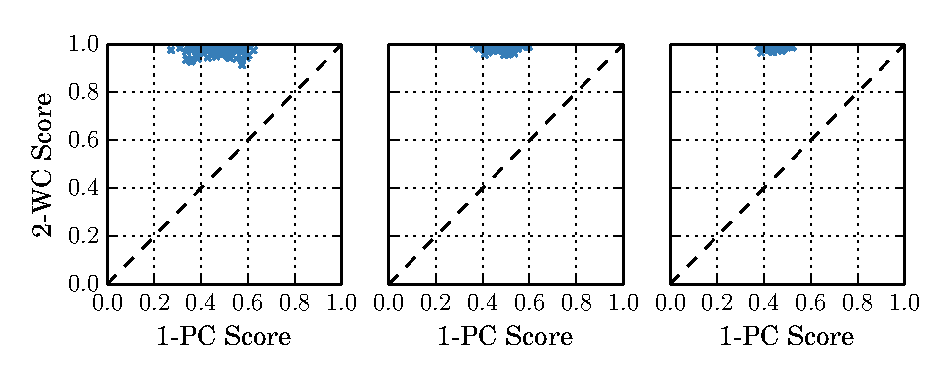
\includegraphics[width=0.49\columnwidth]{figures/ospfresilience2.eps}}
	\subfloat[2-WC vs. 1-WC]
	{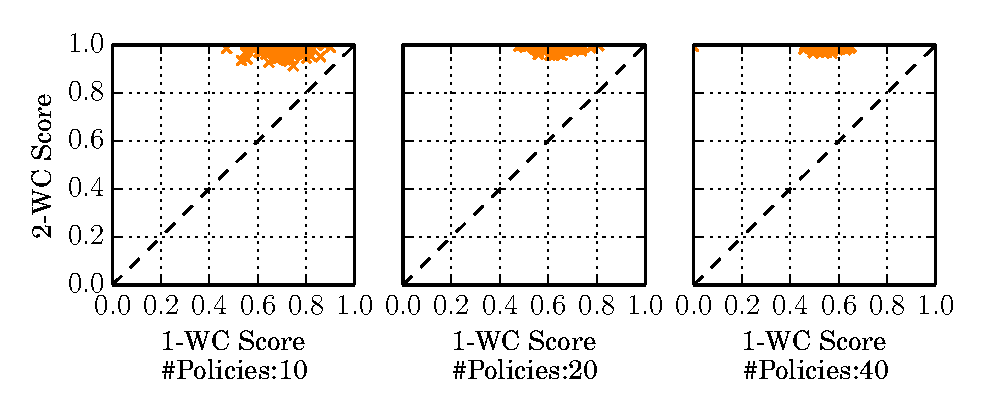
\includegraphics[width=0.5\columnwidth]{figures/ospfresilience.eps}}
	%	\subfloat[Number of Route Filters]
	%	{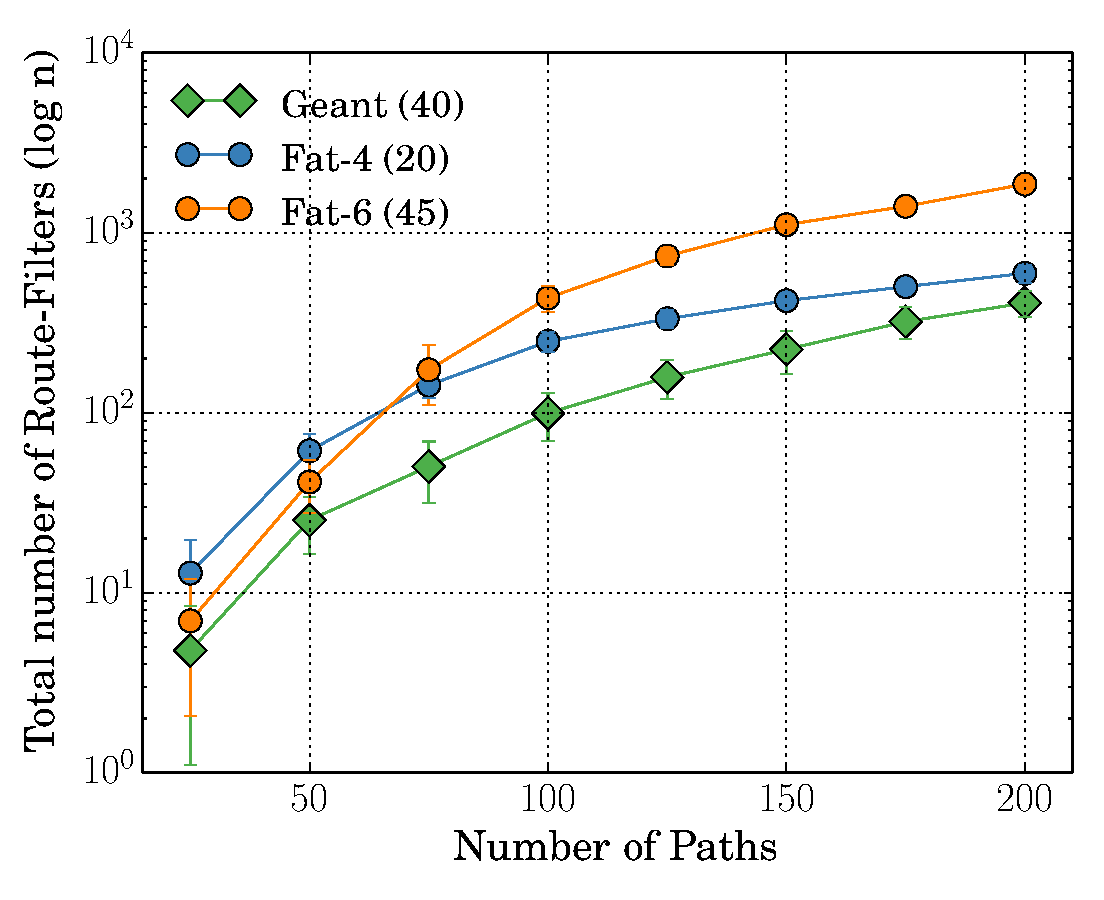
\includegraphics[width=0.33\columnwidth]{figures/ospfRF.eps}}
	%	\subfloat[Endpoint Resilience]
	%	{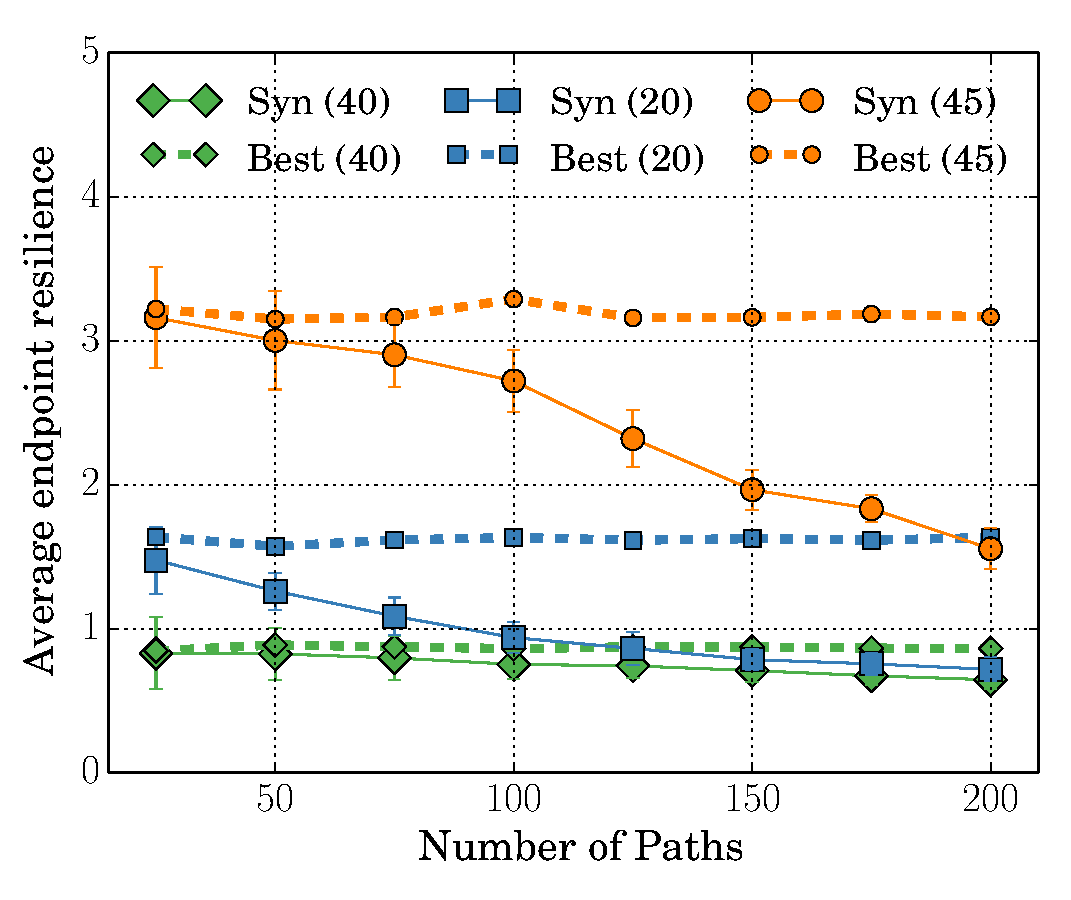
\includegraphics[width=0.32\columnwidth]{figures/ospfAvgRes.eps}}
	\compactcaption{\label{fig:ospfres}
		Policy-resilience scores obtained by 2-WC, 1-WC and 1-PC synthesis 
		for varying waypoint policy workloads.}
\end{figure*}
%\begin{figure*}
%	\centering
%	
%	%	\subfloat[Number of Route Filters]
%	%	{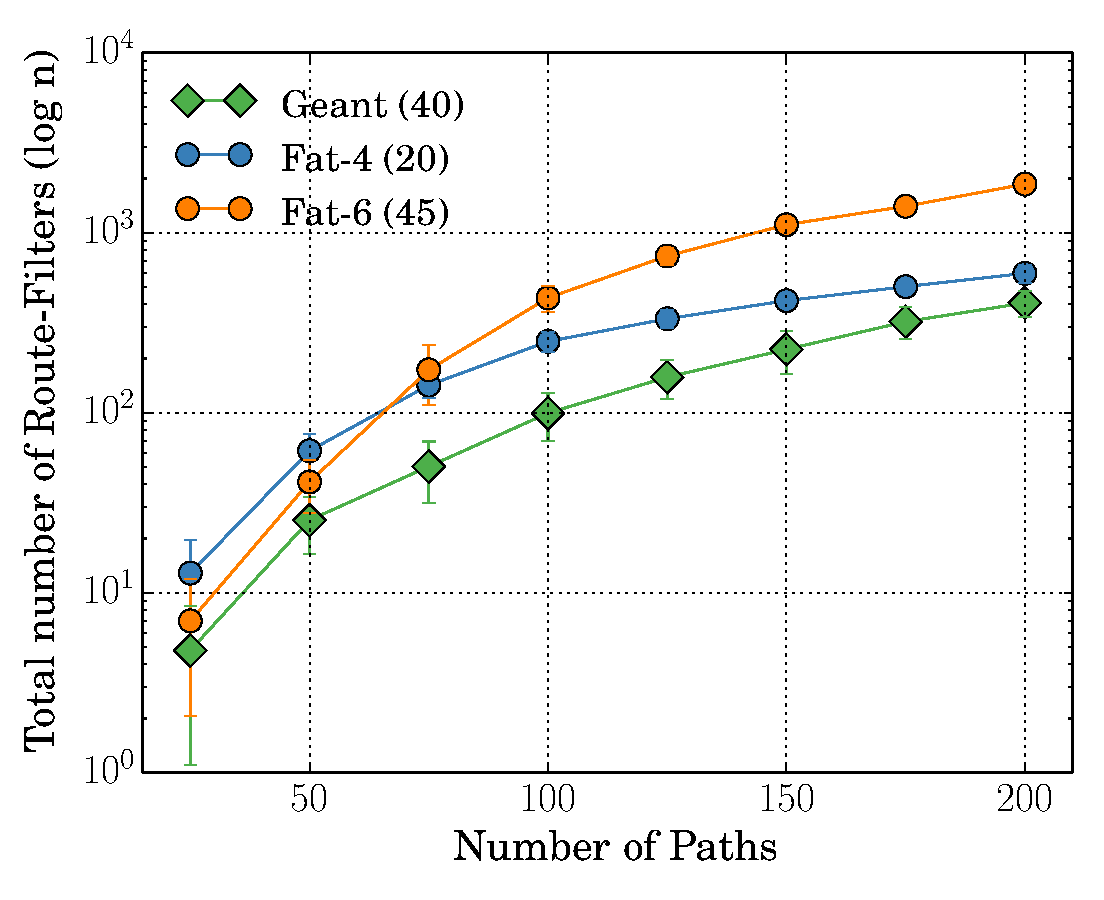
\includegraphics[width=0.33\columnwidth]{figures/ospfRF.eps}}
%	%	\subfloat[Endpoint Resilience]
%	%	{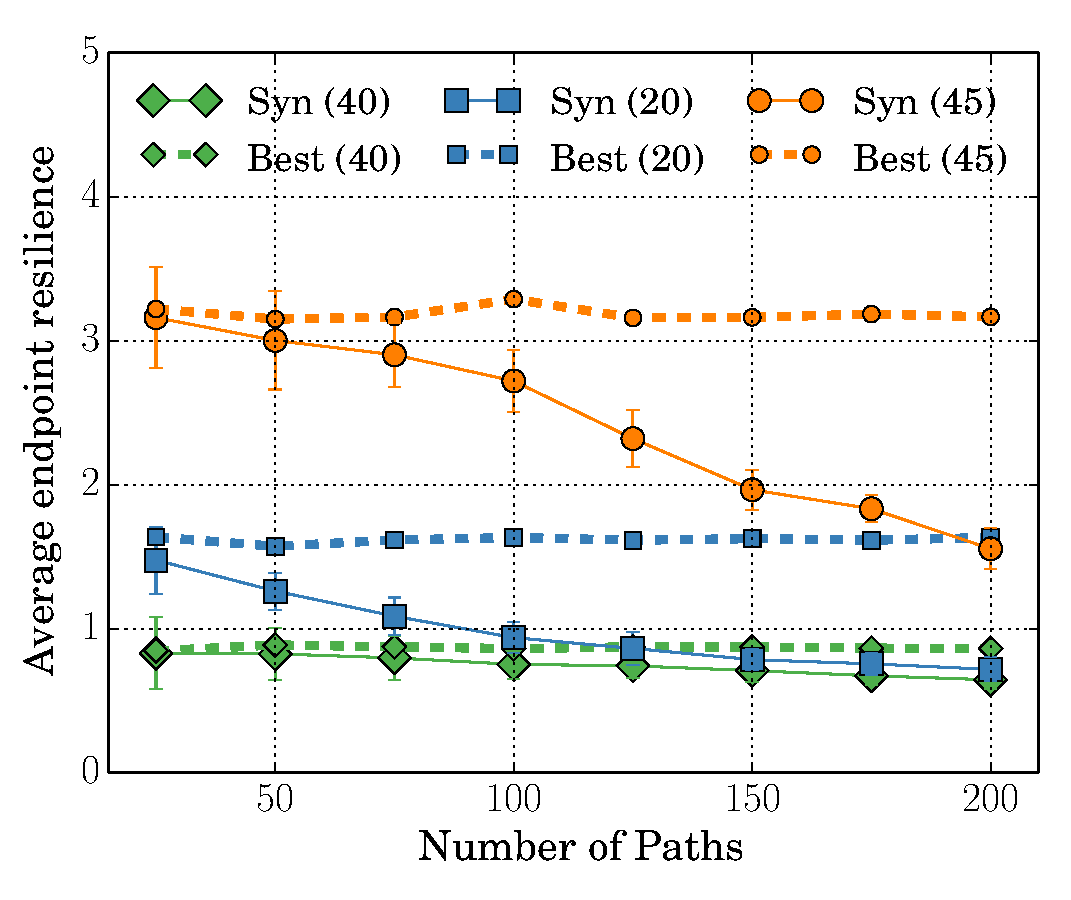
\includegraphics[width=0.32\columnwidth]{figures/ospfAvgRes.eps}}
%	\compactcaption{\label{fig:ospfres}
%		OSPF Synthesis evaluation}
%\end{figure*}


\subsection{Dynamic Domain Assignment Performance} \label{sec:mcmceval}
\begin{wrapfigure}{r}{0.3\columnwidth}
	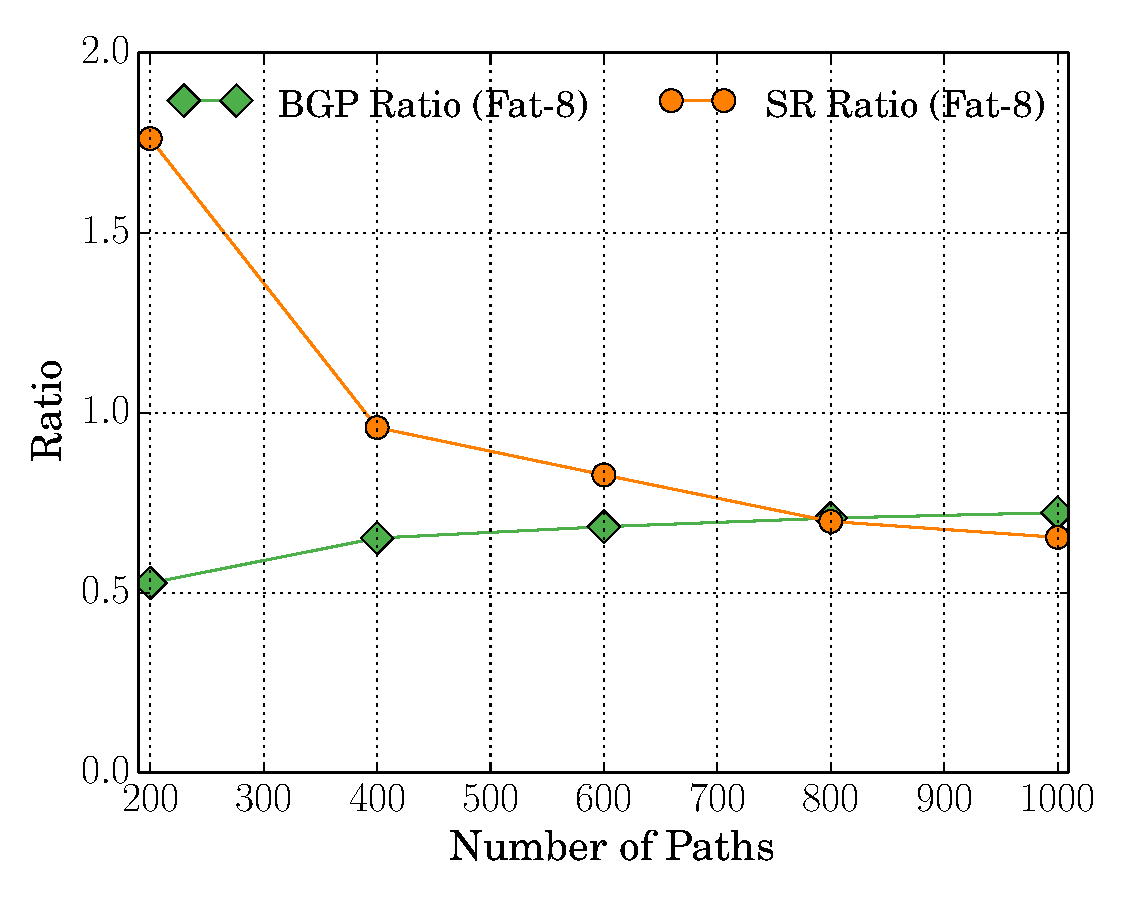
\includegraphics[width=0.29\columnwidth]{figures/ratioMCMC.eps}
	\compactcaption{\label{fig:mcmceval}
		MCMC Evaluation for varying number of paths.}
\end{wrapfigure}

In this section, we demonstrate the advantages of using MCMC sampling
to find a domain assignment which can  
reduce both configuration overhead and number of static routes, 
leading to higher connectivity-resilience. 
For these experiments,
we consider a
80 router fat-tree topology. 
We run the MCMC sampling for 600s
(iterations $>$ 100,000), 
and the tunable parameter $\alpha$ assigning
priority for optimizing configuration 
overhead or static routes is set
to 1. For the input, we generate 
random $n$ paths for $n/4$
destination IPs, with path
 length chosen at random from $[3,10]$. 
We vary $n$ from 200 to 1,000.
We
split the network into 5 OSPF domains 
each with size in range $[10,40]$. We
conduct these experiments 20 times each, 
and report the average and
standard deviation of the metrics.

%\paragraph{Configuration Overhead.}~~~
%\Cref{fig:mcmceval}(a) shows the configuration overhead $bc$ 
%incurred by \name for synthesizing inter-domain configurations.
%For the Fat-8 topology which has greater path diversity, we incur more 
%overhead to ensure path-compliance than the Ion topology. 
%The Best traces indicate the best domain assignment found by MCMC, while 
%Worst traces indicates the domain assignment with greatest 
%configuration cost. 
%This illustrates
%the effectiveness of MCMC sampling in finding configurations with lower overhead on average.
%
%\paragraph{Endpoint Resilience.}~~~ \Cref{fig:mcmceval}(b) shows
%the loss in total endpoint resilience with varying number of paths
%(the count of backup paths for endpoints filtered by the
%configurations). For the Worst traces, we store the worst domain
%assignment in terms of route-filter cost and synthesize the OSPF
%configurations for each domain and calculate the total resilience
%loss. We observe that the MCMC sampling can find domain assignments
%with lower resilience loss than the worst case. This also illustrates
%the effectiveness of the route-filter estimate we use for the cost
%function: a reduction in cost results in greater resilience.
For each MCMC run, we find the best configuration
which optimizes the user-defined quantity based on 
configuration overhead and number of static routes. 
We also store the worst configuration in terms of either
configuration overhead $bc$ and the static route cost 
$sc$. In \Cref{fig:mcmceval}, we plot the average Conf. ratio 
(best configuration overhead/worst configuration overhead), 
the average static route (SR) ratio 
(best / worst number of static routes) and the average 
connectivity-resilence ratio (best/worst connectivity-resilience obtained corresponding to the 
static route cost)
for varying number of paths. 
In smaller workloads, we obtain a 0.5$\times$ reduction, 
but incur an increase in number of static routes. For 
larger workloads, the MCMC sampling is able to
reduce both the static routes 
BGP configuration overhead by $0.3\times$. We also
compare the connectivity-resilience score 
of the best and the worst configuration, and MCMC
is able to increase the connectivity-resilience score 
by $0.1\times$ for large workloads.
%The tunable parameter $\alpha$ 
%can be used to assign different priorities to these objectives to get
%different trends.



